\documentclass{article}

% if you need to pass options to natbib, use, e.g.:
%Enélkül rossz a referencia szamozas!!!!!
\PassOptionsToPackage{square,sort,comma,numbers}{natbib}
% before loading nips_2016
%
% to avoid loading the natbib package, add option nonatbib:
% \usepackage[nonatbib]{nips_2016}

%\usepackage{nips_2016}
\usepackage[final]{nips_2016}

% to compile a camera-ready version, add the [final] option, e.g.:
%\usepackage[final]{nips_2016}

\usepackage[utf8]{inputenc} % allow utf-8 input
\usepackage[T1]{fontenc}    % use 8-bit T1 fonts
\usepackage{hyperref}       % hyperlinks
\usepackage{url}            % simple URL typesetting
\usepackage{booktabs}       % professional-quality tables
\usepackage{amsfonts}       % blackboard math symbols
\usepackage{nicefrac}       % compact symbols for 1/2, etc.
\usepackage{microtype}      % microtypography
\usepackage{graphicx}	%inserting images

%magyar kivonathoz
\usepackage[magyar, english]{babel}

\title{Self-driving vehicle in Duckietown environment\\
	\large Duckpropagation }

% The \author macro works with any number of authors. There are two
% commands used to separate the names and addresses of multiple
% authors: \And and \AND.
%
% Using \And between authors leaves it to LaTeX to determine where to
% break the lines. Using \AND forces a line break at that point. So,
% if LaTeX puts 3 of 4 authors names on the first line, and the last
% on the second line, try using \AND instead of \And before the third
% author name.

\author{
  Attila Pethő
 % \texttt{hippo@cs.cranberry-lemon.edu} \\
  %% examples of more authors
   \And  
   Farkas Olivér István \\
  %% Affiliation \\
  %% Address \\
  %% \texttt{email} \\
   \And
    Faragó Gyula\\
  %% Affiliation \\
  %% Address \\
  %% \texttt{email} \\
  %% \And
  %% Coauthor \\
  %% Affiliation \\
  %% Address \\
  %% \texttt{email} \\
  %% \And
  %% Coauthor \\
  %% Affiliation \\
  %% Address \\
  %% \texttt{email} \\
}

\begin{document}
% \nipsfinalcopy is no longer used

\maketitle

%\selectlanguage{magyar}
%\begin{abstract}
%Kivonat magyarul
%\end{abstract}

%\selectlanguage{english}

\begin{center}
	\large
	\textbf{Abstract}\\
\end{center}
English abstract

\begin{center}
	\large
	\textbf{Kivonat}\\
\end{center}

Magyar kivonat, magyar betűk , üúó

\section{\large{Introduction}}

Self driving vehicles are clearly the future of transportation. If you look at waymo's \cite{waymo}  safety report you can see two things. First it is obvious that AI driven vehicles are more safe than a human driven ones. The other thing which makes development hard is the amount of data needed for the training of the AI. 
The report mentions that the AI used in the cars have learned from over 20 million driven miles. It is quite big number and an astounding achievement given the fact that the car fleet only had 8 bigger accident during this time. The report shows that all accident had a similar cause, human error. In three times the car was stationary and someone ran into it. I think it shows the potential of self driving vehicles.

For us 20 million miles driven seems a lot, but to train well an AI its not that much. This is the reason waymo chosen to train its AI in simulation as well. The driven mile is the simulation were 20 billion. That means in order to archive better results using a simulator is a good idea. Duckietown provides an excellent learning ground for those who want to understand the theory of reinforced learning, and apply the theory in real environment. 
It has started in a class at MIT in 2016. Duckietown has grown so much since then, it's now a worldwide initiative to learn AI and robotics. Our goal was to deep dive into the world of reinforced learning and develop efficient learning strategies for our duckiebots. 

\section{\large{Installation}}

\textbf{Requirements: git installed on your computer}

You need to clone the following repository:\\
\begin{center}
  \url{https://github.com/attila-petho/DuckPropagation}
\end{center}

If you are done with that, change directory into DuckPropagation with the following command:
\begin{center}
	cd DuckPropagation/
\end{center}
After that you need to run the script that sets up the environment:
\begin{center}
	bash env\_setup.sh
\end{center}

\section{\large{Methods}}

\subsection{\normalsize{RL}}

Reinforced learning differs from other machine learning techniques. It can't be put in supervised or unsupervised learning instead it creates its own separate category in machine learning. The reinforced learning model consist of two important element, the environment and the agent (Figure \ref{fig:statemachin}). The environment can be defined as everything that is not the agent and have no total control over it. The environment can be represented mathematically by a set of variables that define each state of the system. The set of all states called state spaces. The agent don't have full access to the state space, it can see only a part of it which is called observation. The agent can modify the current state through actions. The environment reacts to the action with potential state change and a reward.


\begin{figure}[h!]
	\centering
	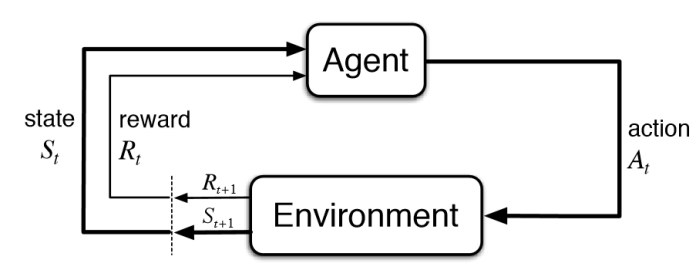
\includegraphics[width=0.8\linewidth]{rl.jpg}
	\caption{Illustration of Reinforcement Learning}
	\label{fig:statemachin}
\end{figure}

The goal is simple, the agent have a predefined task in the environment and must complete it through actions. To archive its goal the agent have to do a three-step process: the agent interacts with the environment, the agent evaluates its behavior, and the agent improves its responses \cite{dlr_book}. The evaluation is based on the previous rewards and the observations. The hardest part is the underlying algorithm in the agent which maps the observation and the rewards to a goal archiving action.

\subsection{\normalsize{A2C, PPO algorithms}}

We tried two promising algorithm for the task: A2C and PPO.The implementation of these algorithms were done by the stable baselines library  \cite{stablebase} so we only had to focus on reward and observation shaping.

\subsection{\normalsize{Environment}}

The environment gives us an 640x480 RGB image.
We have to preprocess this image, because feeding the original images to the CNN would be a waste of resources because it makes training process much slower, and the network can learn from smaller images just as well.

\subsubsection{\normalsize{Observations}}

Preprocessing actions are applied to the observations. These can be resizing the image, cropping the image, grayscale the image, segment the colors in it or stack the last n number of the frames.

\begin{figure}[h!]
	\centering
	\begin{minipage}{.3\textwidth}
	\centering
	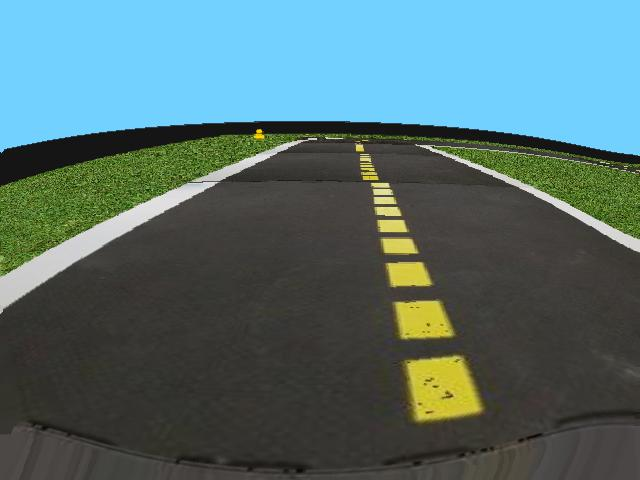
\includegraphics[width=0.8\linewidth]{rawobs.jpg}
	\caption{(a)}
	\end{minipage}%
	\begin{minipage}{.3\textwidth}
	\centering
	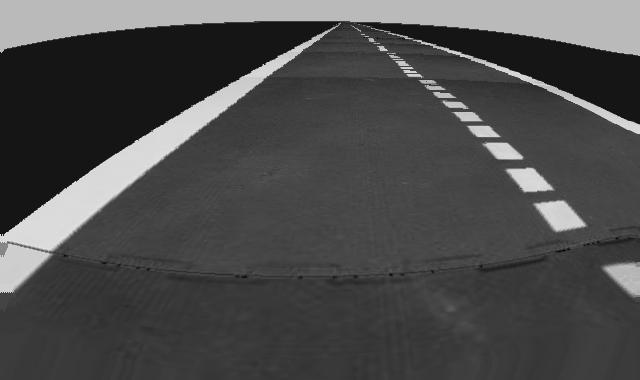
\includegraphics[width=0.8\linewidth]{grayscale.jpg}
	\caption{(b)}
	\end{minipage}%
\begin{minipage}{.3\textwidth}
	\centering
	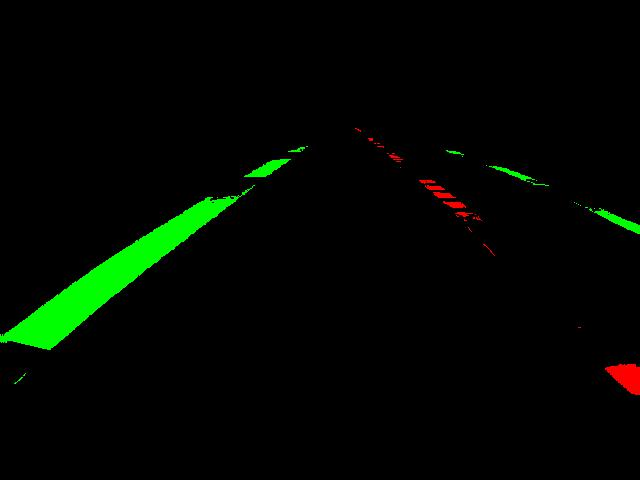
\includegraphics[width=0.8\linewidth]{colorseg.jpg}
	\caption{(c)}
\end{minipage}
\caption{Observations from the environment. (a) shows a raw observation, (b) shows a grayscaled image, (c) shows a color segmentated image}
\end{figure}

\subsubsection{\normalsize{Actions}}

\subsubsection{\normalsize{Rewards}}

\subsection{\normalsize{Evaluation}}

\subsection{\normalsize{Hyperparameter Optimization}}

\section{\large{Results}}

\section{\large{Conclusion}}


\bibliography{bib}
%\addcontentsline{toc}{chapter}{Irodalomjegyzék}
%\bibliographystyle{plain}
\bibliographystyle{ieeetr}
%\bibliographystyle{unsrt}


\end{document}
